%----------------------------------------------------------------------------------------
%	CHAPITRE 1
%----------------------------------------------------------------------------------------
\chapter{Heuristiques de recherche} % Nom du premier chapitre

\label{Chapter1} % For referencing the chapter elsewhere, use \ref{Chapter1} 



%----------------------------------------------------------------------------------------
%	SECTION 1
%----------------------------------------------------------------------------------------
\section{Définitions et intérêt}
Les heuristiques sont des critères, méthodes ou principes utilisées pour sélectionner une solution efficace parmi un ensemble possible afin d'atteindre un ou plusieurs objectifs fixés\cite{judea-pearl-heuristics}.
Elles ne sont d'ailleurs pas toujours justes ou fiables dans toutes les situations et peuvent donc être hasardeuses.

Pour une grande majorité des problèmes complexes, déterminer une solution exacte nécessite d'évaluer un immense ensemble de choix. Le temps requis pour trouver cette solution peut être trop important et il est nécessaire parfois de faire des compromis pour obtenir une solution efficace en un temps raisonnable en utilisant une heuristique. 

Elles sont particulièrement utilisées pour répondre aux problèmes dits NP-complet. Ce sont les problèmes pour lesquels tous les algorithmes connus requièrent un temps exponentiel en pire cas pour être résolus. 
Un des exemples les plus connus et fréquemment enseigné en cours d'algorithmique est le problème du voyageur de commerce.

\subsection{Problème du voyageur de commerce (TSP)}
Soit un ensemble de \textit{n} villes réparties et un voyageur souhaitant toutes les parcourir une et une seule fois puis retourner à la ville d'où il est parti et ce en parcourant au total la distance la plus petite possible.

\begin{center}
    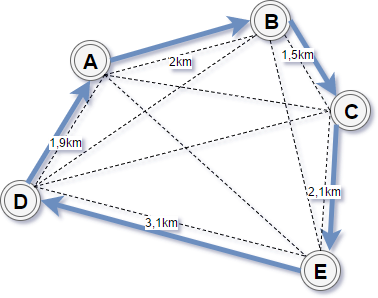
\includegraphics[scale=0.6]{../ressources/images/probleme_voyageur.png}
    \captionof{figure}{Un chemin possible pour résoudre le problème du voyageur de commerce.}
\end{center}

Il existe au total $n!$ chemins possibles soit dans notre cas 120. La ville de départ n'ayant aucune influence sur la longueur totale parcourue on peut donc réduire l'ensemble à $(n-1)!$ soit 24 chemins. Enfin chaque chemin pouvant être parcouru dans les deux sens sans impacter la distance,  on peut donc réduire l'ensemble final à $\frac{1}{2}(n-1)!$ soit 12 chemins.

% Table montrant l'évolution du nombre de chemins en fonction du nombre de villes
\begin{table}[h]
\centering
\begin{tabular}{ l|r }
  Villes & Chemins (solutions) \\
  \hline
  5 & 12 \\
  10 & 181400 \\
  15 & 43 589 145 600 \\
  20 & 60 822 550 204 416 000 \\
\end{tabular}
  \caption{Évolution de l'ensemble des chemins en fonction du nombre de villes pour la résolution du problème du voyageur de commerce}
\end{table}

Le tableau ci-dessus rend compte de la rapidité à laquelle le nombre de chemins à évaluer grandit en fonction du nombre de villes. On parle d'\textit{explosion combinatoire}: c'est le fait qu'un problème se complexifie grandement lorsque le nombre de données à considérer augmente légèrement et peut rendre sa solution incalculable en un temps restreint (longévité humaine par exemple).

\subsection{Un algorithme glouton}
Pour trouver une solution (pas forcément la meilleure) au problème du voyageur de commerce, nous pouvons utiliser une heuristique simple en utilisant un algorithme glouton. Un tel algorithme repose sur le fait de dérouler les données de manière itérative en sélectionnant à chaque étape un optimum local. Ceci a pour effet de grandement diminuer le nombre de données à considérer et donc de répondre en partie à l'explosion combinatoire.

\begin{algorithm}
\caption{Problème du voyageur - un algorithme glouton} 
\label{algo-glouton-TSP}
\begin{algorithmic}
\Function{determiner\_chemin}{$villes, n$}
    \State $P := LISTE\_VIDE$
    \State \textbf{choisir un sommet} u \textbf{dans} villes
    \State $P := P \cup u$
    \While{$|P| \ne n$}
        \State $d := +\infty$
        \For{v \textbf{in} villes}
            \Comment{Évaluation de la ville la plus proche}
            \If{$distance(u, v) < d$}  
                \State $d := distance(c, v)$
                \State $u` := v$
            \EndIf
        \EndFor
        \State $u := u'$
        \State $P := P \cup u$
        \State $villes := villes - u$
    \EndWhile
    \State \Return $P$
\EndFunction
\end{algorithmic}
\end{algorithm}

L'algorithme \ref{algo-glouton-TSP} présente une heuristique simple pour répondre aux problème d'explosion des chemins en diminuant le nombre de données à évaluer. 
Depuis la ville de départ $u$ (choisit aléatoirement par exemple), il s'agit de sélectionner la ville la plus proche parmi les $n-1$ villes restantes. Puis de manière itérative, nous sélectionnons la prochaine ville la plus proche depuis la dernière ville sélectionnée et ceci jusqu'à ce que toutes les villes soient sélectionnées. 
A la première itération nous avons donc $n-1$ distances à évaluer puis nous en aurons $n-2$ à la deuxième. Au final cet algorithme doit évaluer $\frac{n(n-1)}{2}$ distances. 

\newpage

Ceci montre un exemple simple d'utilisation d'une heuristique qui repose sur la découpe du problème en sous-problèmes pour réduire l'ensemble des données du domaine. L'inconvénient est qu'une telle méthode ne donne pas de garantie de résultât car le chemin le plus court possible n'est retourné que dans le meilleure des cas.
La sélection d'une heuristique pour répondre à un problème réside dans le compromis entre le temps requis pour obtenir une solution et la qualité de la solution retournée c'est à dire sa proximité avec la meilleure solution possible. 
Ces deux critères peuvent être évalués en moyenne, dans le pire cas possible, dans le meilleure cas possible ou bien les trois à la fois. \\

% Table montrant l'évolution du nombre de chemins en fonction du nombre de villes
\begin{table}[h]
\centering
\label{table-comparaison-chemins}
\begin{tabular}{ l|r|r }
  Villes & Chemins & Chemins (algorithme glouton) \\
  \hline
  5  & 12                     & 10  \\
  10 & 18 1400                & 45  \\
  15 & 43 589 145 600         & 105 \\
  20 & 60 822 550 204 416 000 & 190 \\
\end{tabular}
  \caption{Comparaison du nombre de chemins évalués pour la résolution du problème du voyageur de commerce avec un algorithme glouton (heuristique).}
\end{table}

Les heuristiques sont intéressantes en dehors du domaine théorique car la majorité des problèmes pratiques ne nécessite pas d'établir la solution la plus optimale. On préférera trouver un équilibre entre la qualité de la solution obtenue et le coût pour trouver une telle solution qui est un critère non négligeable si l'on prend compte du contexte économique. On parle alors de problème de \textit{semi-optimisation} et plus particulièrement d'optimisation proche lorsque qu'il s'agit de trouver une solution dans un intervalle de coût définie ou de problème d'optimisation approximatif lorsqu'il s'agit de se rapprocher de l'optimum avec une probabilité importante.

%TODO Paragraphe de transition

% SOUS-SECTION 2
\section{Modélisation}
Pour établir une bonne heuristique et évaluer sa capacité à produire des solutions en un temps défini sur un problème donné, il convient de correctement le représenter.
De nombreux problèmes peuvent être formulés comme problème de satisfaction de contraintes - où l'on cherche des états ou des objets satisfaisant un certain nombre de critères - et d'optimisation de tâches. De plus, une heuristique doit pouvoir être automatisée et donc être résolu à l'aide des machines actuels.

Puisque toutes les recherches de solutions à un problème peuvent se résumer à la tâche de construire un object avec les caractéristiques données, les besoins\cite{judea-pearl-heuristics} pour la résolution avec un ordinateur sont les suivants:

\begin{enumerate}
\item Une structure de symbole appelée code ou base de données représentant les sous-ensembles des solutions potentielles.
\item Un ensemble d'opérations ou des règles de production qui modifient les symboles de la base de données pour produire un sous-ensemble de solutions plus fins ou précis.
\item Une procédure de recherche ou stratégie de contrôle qui décide quelles opérations sont à appliquer sur la base de données.
\end{enumerate}

\subsection{Définitions générales}
Les différentes façons de représenter nos problèmes repose majoritairement sur des modèles de graphe. Vous pouvez passer à la section suivante si vous possédez déjà des connaissances de base de théorie des graphes sinon nous décrivons brièvement les notions importantes ici:\\

{\setlength{\parindent}{0cm}\textbf{Graphe:}}

Un graphe est composée d'un ensemble de \textbf{nœuds} ou \textbf{sommets} reliés par des \textbf{arcs} ou \textbf{arêtes} pouvant être associées à des valeurs (par exemple la distance entre deux sommets) ou bien être dirigé (donnant la direction, on va d'un nœud à l'autre).
Dans notre cas, nos graphes auront toujours un nœud de départ appelé \textbf{nœud racine}.
L'ensemble des nœuds est le plus souvent noté $V$ et on note $E$ pour l'ensemble des arêtes du graphe. 
Un graphe est mathématiquement représenté de cette façon: $G = (V, E)$.
Le \textbf{degré} d'un sommet est le nombre d'arêtes de celui-ci.\\

\begin{center}
    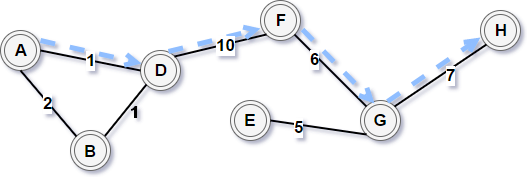
\includegraphics[scale=0.6]{../ressources/images/example_graph.png}
    \captionof{figure}{Représentation d'un graphe à 7 sommets et 7 arêtes avec un chemin dessiné en bleu entre le sommet A et le sommet H: \{A, D, F,G, H\}.}
\end{center}

{\setlength{\parindent}{0cm}\textbf{Arbre:}}

Un arbre est un graphe non orienté dans lequel chaque nœud (sauf le nœud racine) n'a qu'un seul parent. 
On désigne comme \textbf{feuille} un nœud n'ayant aucun fils.
Dans un arbre on définit la \textbf{hauteur} comme étant la longueur du chemin de la racine vers le nœud feuille le plus éloigné. On parle de \textbf{profondeur} quand il s'agit de la distance entre n'importe quel nœud feuille et le nœud racine.
On parle d'\textbf{arbre uniforme} pour désigner un arbre fini de hauteur $n$ dont tous les nœuds qui sont inférieur en profondeur à $n$ ont le même degré et où tous les nœuds de profondeur $n$ sont des feuilles.

\begin{center}
    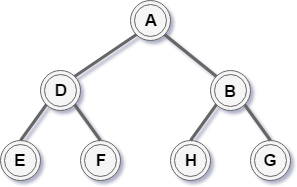
\includegraphics[scale=0.6]{../ressources/images/example_tree.png}
    \captionof{figure}{Un arbre uniforme de profondeur 2 à 7 sommets et 6 arêtes}
\end{center}

%TODO (P.34) Regarder si c'est utile, peut être le déplacer. 
%{\setlength{\parindent}{0cm}\textbf{Recherche dans un graphe:}}
%Dans notre cas, nous recherchons des heuristiques pour répondre à l'explosion combinatoire et donc dans le cas d'une représentation sous forme de graphe nous pouvons aussi parler d'explosion des chemins. L'ensemble des données est parfois tellement importante qu'il est impossible de modéliser l'ensemble.
%Pour combler ces lacunes, il est possible d'utiliser des techniques de génération du graphe pas à pas.

% Beaucoup de problèmes sont décrits comme des tâches pour chercher des propriétés sur un graphe.
% Objectif: Trouver des méthodes efficaces pour trouver la solution rapidement dans le graphe.

Le choix d'une représentation pour encadrer un problème se fait en fonction des contraintes et des données mais ce choix n'est pas unique et peut être différent en fonction de l'approche souhaité.

\subsection{ET-OU graphe}
Le graphe \textit{ET-OU} (ou graphe de réduction de problème) est une modélisation destinée à représenter un problème comme étant la conjonction de plusieurs sous-problèmes qui peuvent être résolus indépendamment.
Cette représentation est principalement utilisée lorsqu'il s'agit de trouver une stratégie de recherche efficace, c'est par exemple le cas si l'on souhaite résoudre le problème de la pièce contrefaite:

Nous avons douze pièces de monnaie et parmi elles se trouve une pièce contrefaite, c'est à dire qui est soit plus légère ou plus lourde que les autres. L'objectif est de déterminer une stratégie pour identifier en au plus trois pesées (avec une balance) quelle est la pièce contrefaite. Il s'agit donc de sélectionner une suite d'actions de ce qui doit être pesé en premier pour avoir une chance d'identifier la pièce contrefaite.
Bien entendu, ce problème peut être résolu en énumérant la totalité des solutions possibles mais l'objectif ici est d'utiliser une heuristique pour identifier une stratégie qui permette de résoudre ce problème en un minimum de pesée (action).

Pour résoudre ce problème, il faut décider du nombre de pièces à comparer à chaque pesée. On peut par exemple décider de peser les pièces une à une, deux à deux, trois à trois, et ainsi de suite. Intuitivement, on sait que si à la première action l'on compare un sous-ensemble de pièces restreint en prenant seulement deux pièces, l'approche sera plus hasardeuse puisqu'à la prochaine action, le sous-ensemble restant risque d'être trop important pour identifier une pièce contrefaite. 
Par contre, si nous pesons deux pièces au hasard en premier, il est possible d'obtenir le résultât en une seule pesée si l'une des deux est soit plus légère ou plus lourde.

Dans ce problème, nous ne sommes pas que confronté au choix de la prochaine action à entreprendre mais aussi aux conséquences de celle-ci qui affecteront inévitablement les prochaines décisions et délimiterons le prochain sous-ensemble.

Pour cela nous utilisons donc le graphe de réduction de problème où les nœuds représentent les sous problèmes et les arcs les conséquences de l'action entreprise sur ce sous-problème. L'avantage de ce type de modélisation est qu'il permet de découper le problème initial en sous-problèmes indépendants grâce à une technique appelée « diviser pour régner ».\\

{\setlength{\parindent}{0cm}\textbf{Arêtes ET:}}

Mène à des sous-problèmes indépendants qui devront tous être résolus pour résoudre le problème associé au nœud père. Cet arc représente les changements dans la situations du problème.\\

{\setlength{\parindent}{0cm}\textbf{Arêtes OU:}}

Mène à des sous-problèmes alternatifs, dont l'un devra être résolu pour résoudre le problème associé au nœud père. Cet arc représente les différentes réactions possible après un tel changement.

\begin{center}
    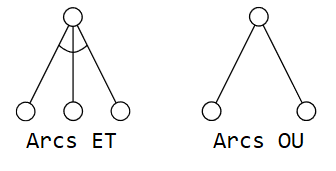
\includegraphics[scale=0.8]{../ressources/images/ET_OU_arcs.png}
    \captionof{figure}{Respectivement les arcs ET et OU du graphe de réduction de problème.}
\end{center}

Nous pouvons donc modéliser notre problème sous forme de graphe où chaque décision prise depuis le nœud racine forme une solution possible résultant de la première action entreprise. Une solution n'est pas donc qu'un chemin dans le graphe, mais un sous-graphe de notre modèle commençant au nœud racine. La figure 1.5 donne un exemple d'une solution possible où l'action de comparer 2 pièces de monnaies est prise en premier.

\begin{center}
    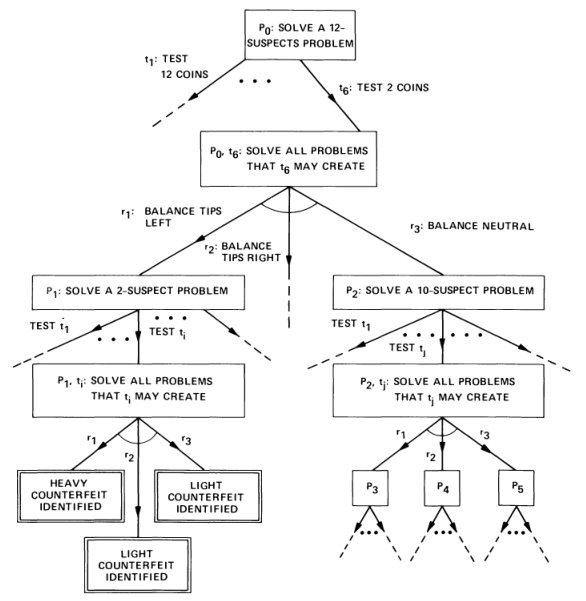
\includegraphics[scale=0.8]{../ressources/images/counterfeit_problem_and_or_graph.png}
    \captionof{figure}{Problème de la pièce contrefaite représenté avec un ET-OU graphe\cite{judea-pearl-heuristics}}
\end{center}

%TODO Conclure + transition

\subsection{Représentation d'état}
Une représentation d'état consiste essentiellement en un ensemble de nœuds représentant chacun les états possibles du problème. Les arêtes entre les nœuds représentent les actions possibles d'un état à un autre. 
Chaque représentation d'état prend la forme d'un graphe ou d'un arbre.

Une représentation sous forme d'espaces états sera plutôt utilisé pour modéliser un problème de satisfaction de contraintes ou de recherche de chemin.
Si la solution peut être exprimée comme une séquence d'actions inconditionnelles ou comme un seul objet avec un ensemble de caractéristiques nous avons un problème de plus court chemin ou de satisfaction de contraintes qui est donc modélisable comme ceci.

Avant de représenter notre problème, il faut préalablement définir un ensemble de facteurs:
\begin{itemize}
\item Quel est l'objectif à atteindre ?
\item Quels sont les actions possibles ?
\item Quels informations doivent être représentées dans la description des états ?
\end{itemize}

Par exemple on peut souhaiter rechercher des erreurs dans un programme. Pour cela, nous pouvons modéliser chaque nœud comme étant un état du programme issu des différentes conditions de branchement où les valeurs concrètes en mémoire seraient remplacées par des valeurs symboliques. Il s'agit alors de parcourir le graphe, pour identifier d'éventuelles valeurs pour lesquelles le programme n'aurait pas le comportement souhaité.

\begin{center}
    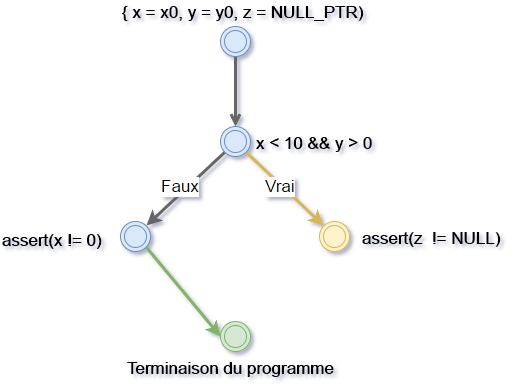
\includegraphics[scale=0.6]{../ressources/images/state_space_graph.png}
    \captionof{figure}{Représentation sous forme d'état de l'exécution symbolique d'un programme}
\end{center}

%TODO (P.34) Définir toutes les notions pour l'explorations des noeuds
%Noeud étendu: Génération de tous les successeurs d'un noeud parant (mais pas les successeurs des successeurs je crois).
%Noeud exploré: Noeud visité
%Noeud généré: Génération d'un noeud successeur à partir de sont parant.